\documentclass{article} % For LaTeX2e
\usepackage{nips11submit_e,times}
\usepackage{graphicx}
\usepackage{wrapfig}
%\documentstyle[nips10submit_09,times,art10]{article} % For LaTeX 2.09


\title{Modeling Fly Trajectories to Automatically Detect Mutations}


\author{
Joseph Marrama \\
Department of Symbolic Systems\\
Stanford University\\
\texttt{jmarrama@stanford.edu} \\
\And
Alden Timme \\
Department of Math and Computational Sciences \\
Stanford University \\
\texttt{aotimme@stanford.edu} \\
}

\newcommand{\fix}{\marginpar{FIX}}
\newcommand{\new}{\marginpar{NEW}}

\nipsfinalcopy % Uncomment for camera-ready version

\begin{document}


\maketitle

%is an abstract necessary?
%\begin{abstract}
%\end{abstract}



\section{Introduction}
%a bit on the problem at hand... not too long

In biological experiments involving flies, making sure all the flies that are assumed to be normal actually are healthy wildtype flies is of the utmost importance. There have been previous studies on normal and mutated flies that suggest there is a way to automatically classify flies as normal or not given measurements of their movements. These studies have produced a great deal of observational data of fly movements as well. In our project, we use this data to develop a model that performs reasonably well on automatically classifying flies as healthy or mutated.


\section{Related Work}
%what the fuck? are you serious? i've certainly read a fuckload about classifying flies, give me a goddamn break daphne
%the project guidelines says we have to put this in.....


\section{Our models}
%uh...... i guess we explain our models here? The guidelines say to include a section about 'our implementation', so i guess this is it. 

%Question: different subsection for different models and then present their performances in 'results', or should we just go through chronologically what we tried and how we iterated through better and better models, presenting the results of each one after its description?

The data in this project is presented as a set of measurements along a number of trajectories of walking flies. We are presented with trajectories for both wild type (normal) flies and for mutated flies. Along these trajectories we are provided a number of measurements, taken at intervals of $1/30$ of a second. These measurements are translational velocity in the forward direction (VT), translational velocity in the sideways direction (VS), rotational velocity (VR), the fly orientation (PO), the fly position along the x-axis (PX), and the fly position along the y-axis (PY). The other important data are the stimulation pulses. There are two types of motion stimuli, corresponding to coherent random dot motion in one direction ($S_1$) and coherent random dot motion in the opposite direction ($S_2$). $S_1$ and $S_2$ are presented in pulses that last either 4 or 5 time steps (where a time step is $1/30$ of a second), and when no stimulus is applied there is a constant noise of random, incoherent dot motion. In addition, these experiments were carried out in 3 different conditions. The three conditions are ?decrement?, in which dark dots are presented over a bright background; ?increment?, in which bright dots are presented over a dark background; and ?dark?, in which noise was replaced by a medium light level and the only stimulus was a dark pulse (complete darkness).

Because this data belongs to a time series, our approach was to design a temporal probabilistic graphical model to model the trajectories of the wild type flies. After training a model on normal flies, we use it to identify wild-type or mutant flies by assigning a log-likelihood to a trajectory (given the model) and assuming that a fly is mutant if the log-likelihood is too low and is wild-type if the log-likelihood is high enough. However, because the trajectories are of different lengths (trajectories last from 20 up to 200 time steps), we choose as our metric the log-likelihood of the trajectory divided by the length of the trajectory (the trajectory?s average log-likelihood). We use the average log-likelihood for identifying wild-type and mutant flies by using a validation data set (of wild-type and mutant flies) to find the best average log-likelihood cut-off. Anything below this cut-off is determined to be mutant and everything above is wild-type. The best average log-likelihood cut-off is the average log-likelihood that maximizes the $F_1$ score,
\begin{eqnarray*}
F_1 &=& \frac{2\cdot precision \cdot recall}{precision + recall}\\
precision &=& \frac{tp}{tp + fp}\\
recall &=& \frac{tp}{tp + fn}
\end{eqnarray*}
where $tp$ is the number of true positives, $fp$ is the number of false positives, and $fn$ is the number of false negatives. To see an example of a the $F_1$ score graphed as a function of the average log-likelihood of a validation set, see Figure 3.

The data on fly positions (PX and PY) were confounding because they were not calibrated, so our models considers only the velocities, VT, VS, and VR, the orientation, PO, and the stimuli, $S_1$ and $S_2$. The first few measurements on each trajectory are very obviously way off, so we throw out the first 6 time steps of each trajectory. We also need a way to represent the stimuli in our model. Although the stimuli are applied in pulses, there is evidence showing that the effects of the pulses on the flies will last a few time steps after the pulse ends (REF). However, we do not expect the stimulus to affect the fly many time steps after the last pulse, so we parameterize the variables $S_1$ and $S_2$ (corresponding to the two stimulus types) by the amount of time since the beginning of the most recent pulse. The value 1 corresponds to the beginning of a new pulse, and at each time step thereafter will be $2, 3, \ldots$ until reaching a maximum value of $M$ (the fly has limited memory after all). Once we are past M time steps after the pulse, the value of $S_i$ ($i=1,2$) is $0$. This way of encoding the stimulus allows the model to take into account an M-order Markovity of the time series.

Our first model is a baseline model, where each variable at a given time-step $\tau$ is dependent only on the same variable at the time-step $\tau-1$ and the stimuli $S_1, S_2$ at the current time step $\tau$ (Figure 1). The probability distributions are parameterized by linear Gaussians,
\begin{eqnarray}
P(X^{\tau} = x^{\tau} | X^{\tau-1}=x^{\tau-1}, S_1, S_2) \sim \mathcal{N}\left( \theta_{x,0} + \theta_{x,1}S_1 + \theta_{x,2}S_2 + \theta_{x,3}x^{\tau-1}, \; \sigma_x \right)
\end{eqnarray}
where $X^{\tau}$ is one of the four observed variables at time step $\tau$.
However, because the orientation variable (PO) takes on values in $[-\pi,\pi]$, this model can run into problems in the region around $-\pi$ and $\pi$, which are the same orientation but have very different parameterizations. To deal with this, we split up the orientation variable into the cosine and sine of the variable (cO and sO, respectively), and connect cO and sO at each time step to both cO and sO at the next time step (Figure 1).

We also try a fully connected model in which every observed variable at time step $\tau$ (except the stimulus variables) is distributed according to a linear Gaussian, where the mean is a linear combination of all the observed variables at time $\tau-1$ (except the stimuli) and the stimuli variable at time $\tau$ and the variance depends only on the variable (Figure 1). We try this both with the orientation variable left as is and with the orientation variable split into its sine and cosine (Figure 1).

\begin{figure}[t]
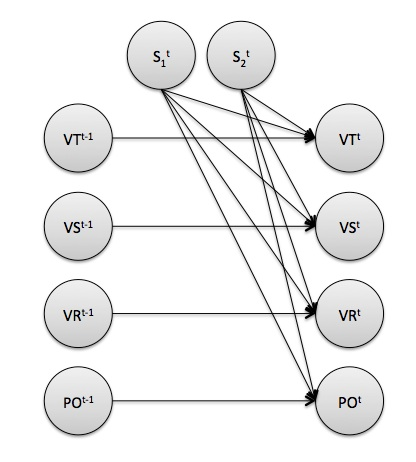
\includegraphics[width=3.5cm]{simple.jpg}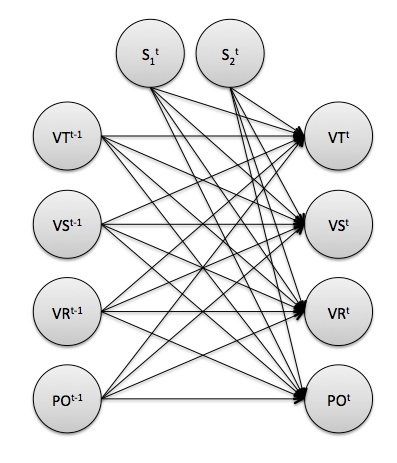
\includegraphics[width=3.5cm]{full.jpg}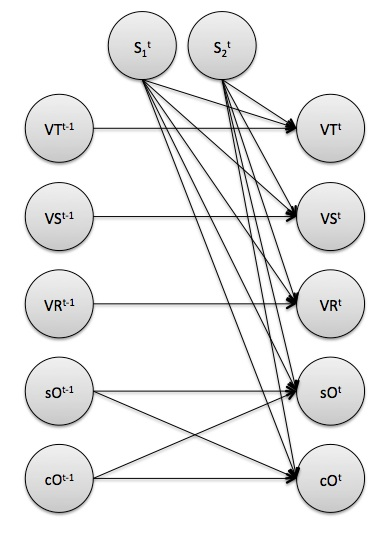
\includegraphics[width=3.5cm]{simple-sincos.jpg}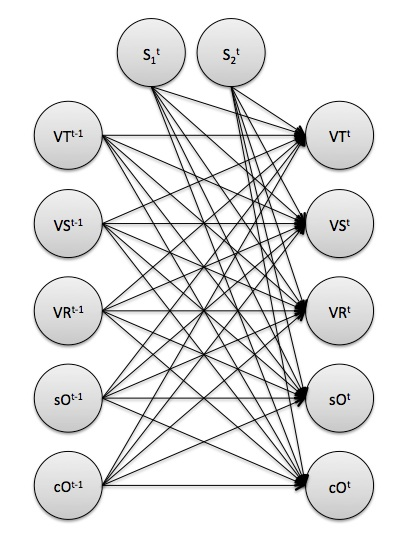
\includegraphics[width=3.5cm]{full-sincos.jpg}\\
\caption{From left to right: (a) simple connected model, (b) fully-connected model, (c) simple connected model with orientation split into $sin$ and $cos$, and (d) fully-connected model with orientation split into $sin$ and $cos$} % have to figure out where to put this figure...
\end{figure}

Finally, we have one more model which makes use of hidden variables. In this model, all of the observed variables (i.e. measurements) at each time step depend only on a hidden variable in that time step. This hidden variable $Z$ depends on the hidden variable at the previous time step and the stimuli at the current time step. For each pair $(S_1,S_2)$, we learn a transition matrix from each state $z$ to every other state $z?$. The observed variables at each time step are distributed normally with a mean and variance depending on the hidden state (Figure 2). The motivation for this model is that flies will often initiate a ``move" that will last a number of time steps. This move is probably based on the fly's previous move and the stimuli, so we use the hidden variable as a way of trying to encode a fly's move.

\begin{wrapfigure}{r}{0.5\textwidth}
  \begin{center}
    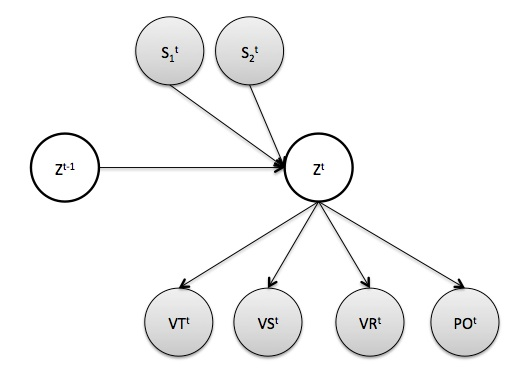
\includegraphics[width=5cm]{hidden.jpg}
  \end{center}
  \caption{Model with a hidden ``move" variable $Z^\tau$}
\end{wrapfigure}

\normalsize
We use the Expectation-Maximization Algorithm to learn the parameters for the hidden model. In order to learn the expected sufficient statistics during the E-step, we tried exact and approximate inference techniques. To infer exactly, we use a variant of the forward-backward equations commonly used to learn hidden Markov models (HMMs) to efficiently provide a distribution over all possible hidden state sequences for each trajectory.

Letting $O^{(\tau)}$ represent the set of observations $VT^{(\tau)}, VS^{(\tau)}, VR^{(\tau)}, PO^{(\tau)}$, we have the set of forward-backward equations,
\begin{eqnarray*}
\gamma(z^{(\tau)}) &=& \frac{\alpha(z^{(t}) \beta(z^{(\tau)})}{P(O^{(1:T)})}\\
\alpha(z^{(\tau)}) &=& P\left(O^{(\tau)} | z^{(\tau)}\right) \sum_{z^{(\tau-1)}} \alpha(z^{(\tau-1)}) P\left(z^{(\tau)} | S_1^{(\tau)}, S_2^{(\tau)}, z^{(\tau-1)}\right)\\
\beta(z^{(\tau)}) &=& \sum_{z^{(\tau+1)}} \beta(z^{(\tau+1)}) P\left(O^{(\tau+1)} | z^{(\tau+1)}\right) P\left(z^{(\tau+1)} | z^{(\tau)}, S_1^{(\tau+1)}, S_2^{(\tau+1)}\right)
\end{eqnarray*}
so that $\gamma(z^{(\tau)})$ normalized represents the probability that a particular value is the true value of the hidden state at time step $\tau$. These weights are used for learning the Gaussian parameters for the model. The transition probabilities from a state $z$ at $\tau-1$ to $z'$ at $\tau$ given the stimuli $S_1$ and $S_2$ at $\tau$ are found by normalizing the expected sufficient statistics provided by:
\begin{eqnarray*}
\xi(S_1, S_2, z^{(\tau-1)}, z^{(\tau)}) &=& \frac{\alpha(z^{(\tau-1)})P(o^{(\tau)} | z^{(\tau)}) P\left(z^{(\tau)} | z^{(\tau-1)}, S_1^{(\tau)}, S_2^{(\tau)}\right) \beta(z^{(\tau)})}{P(O^{(1:T)})}
\end{eqnarray*}

For approximate inference, we used the technique of particle filtering, sending about 1000 particles through each trajectory to obtain an approximate distribution over state sequences for the trajectory. We then were able to measure the expected sufficient statistics from the empirical probability distribution provided by averaging over each of the time steps for all of the final particles on each trajectory.

\normalsize
\section{Results}
\begin{table}[t]
\caption{$F_1$ scores with different models}
\begin{center}
\begin{tabular}{l|ccc|ccc}
 & & Increment & & & Decrement & \\ \hline
  & $F_1$ & Precision & Recall & $F_1$ & Precision & Recall \\ \hline
 Simple & $0.7143$ & $0.5926$ & $0.8989$ & $0.7003$ & $0.5633$ & $0.9253$ \\
 Simple - split & $0.7360$ & $0.6393$ & $0.8671$ & $ 0.7193$ & $0.6094$ & $0.8776$ \\
 Full & $0.7156$ & $0.5944$ & $0.8988$ & $0.7194$ & $0.5642$ & $0.9254$ \\
 Full - split & $0.7356$ & $0.6431$ & $0.8618$ & $0.7194$ & $0.6089$ & $0.8787$ \\
 Hidden - LL & $0.6930$ & $0.5300$ & $1.0000$ & $0.6969$ & $0.5348$ & $1.0000$ \\
 Hidden - TopLL & $0.7270$ & $0.6210$ & $0.8760$ & $0.7119$ & $0.5936$ & $0.8892$
\end{tabular}
\end{center}
\end{table}
%see my question above
The results from all of our models are shown in Table 1. As we can see, the models all do much better at recall than precision. This is probably because the models do not provide enough separation between the two average log-likelihood distributions. Therefore, maximizing the $F_1$ favors maximizing the recall, which is relatively easy to do by decreasing the cut-off log-likelihood to include more true positives. Figure 3 provides an example of the $F_1$ score as a function of the log-likelihood (graphed on a validation set) for the baseline model with the orientation variable split into its sine and cosine (Simple - split in Table 1). As we can see, the $F_1$ is constant for lower values of the log-likelihood, followed by a small hump and a quick plummeting. This hump represents the very small amount of separation between the two distributions (of wild-type flies and mutant flies) with the model. All of our models have graphs that look very much like this one.

Our first baseline (simple) model, where each variable only depends on the same variable in the previous timestep and the stimuli, performed quite well. With just the minor change of splitting the orientation (PO) variable into its sine and cosine, we achieved the highest $F_1$ on the Increment data set. The minor change also allowed it to perform among the best models on the Decrement data set. 

Our next models are simply extensions of the previous two. They are the baseline models with full connections across time steps. That is, every observed variable in time step $\tau$ depends on every observed variable in time step $\tau-1$ (except the stimuli), and the stimuli in time step $\tau$. These models, as we can see in Table 1, perform almost identically to their singly-connected counterparts. This suggests that the observed variables are probably independent of each other given the stimuli. In fact, when looking at the parameters of the linear Gaussians for fully-connected models, parameters for variables other than the child had coefficients very close to zero.

As a note, the log-likelihoods of the trajectories are often positive, because the probability density function of a normal distribution (our models use Gaussians and linear Gaussians) can be greater than $1$. This will occur when the variance of the distribution is very small and we are evaluating the pdf at a point close to the mean of the distribution. Thus it is not so much of a surprise that the optimal average log-likelihood cut-offs were  around $2.5$ on the Increment data on models that did not split the orientation variable and $6.6-6.7$ on models that did. Similarly, for the Decrement data, models that split the orientation variable had optimal cut-offs around $1.7$ and models that did not split the variable had optimal cut-offs around $6.2$.

\begin{figure}[t]
  \begin{center}
	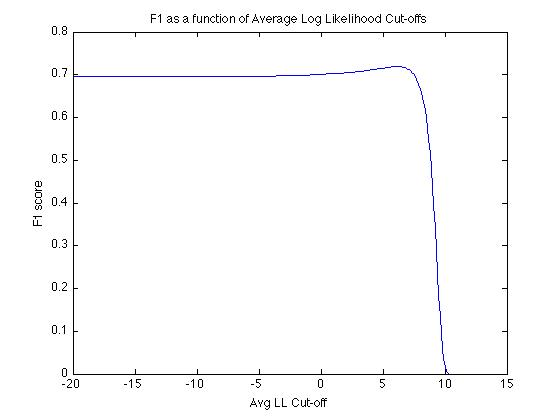
\includegraphics[width=10cm]{simple-sincos-llf1.jpg}
	\end{center}
	\caption{The $F_1$ score as a function of the average log-likelihood cut-off (for the simple model with the orientation variable split into its sine and cosine).}
\end{figure}

\section{Discussion}
%smallden is in the dept. of ball sucking, LOL
Initially, the most surprising result we found was that the stimulation really had no effect on all of our models. Looking through the parameters learned for all of our models, the ones that control the stimulation�s affect on other variables were often near-zero, or very similar across all values of $S_1$ and $S_2$. For example, in all four of our models without hidden variables (see Figure 1), the parameters $\Theta_{x,1}$ and $\Theta_{x,2}$ in Eqn. 1 are always near-zero. In our models with hidden states, $P(z^{\tau}|z^{\tau-1},s_1^{\tau} = i, s_2^{\tau} = j)$ is almost always near-equal to $P(z^{\tau}|z^{\tau-1},s_1^{\tau} = k, s_2^{\tau} = k)$, for all $i$, $j$, $k$, and $l$. To test this, we simply made a variant of our single-conneciton baseline model with cO and sO and excluded the variables $s_1$ and $s_2$. Lo and behold, the model got almost identical $F_1$, precision, and recall scores. 

We believe that this may be more indicative that flies are generally unaffected by the stimuli, rather than that our models fail to account property for the stimuli. Of all the variables that might be affected by a stimuli, the three different components to the fly�s velocity and its orientation seem to be the most likely candidates for changing during or after stimulation. Also, all stimuli only last 4 or 5 timesteps, which corresponds to a sixth of a second or less. This may not be long enough to affect the fly. It would be an interesting continuation of this project to run statistical analysis on the dataset to figure out whether there is any correlation between $S_1$ or $S_2$ and the rest of the variables. 


\end{document}
